\section{Get me on, Get me off}

At first the enhanced schema

\begin{figure}[htbp]
  \centering
  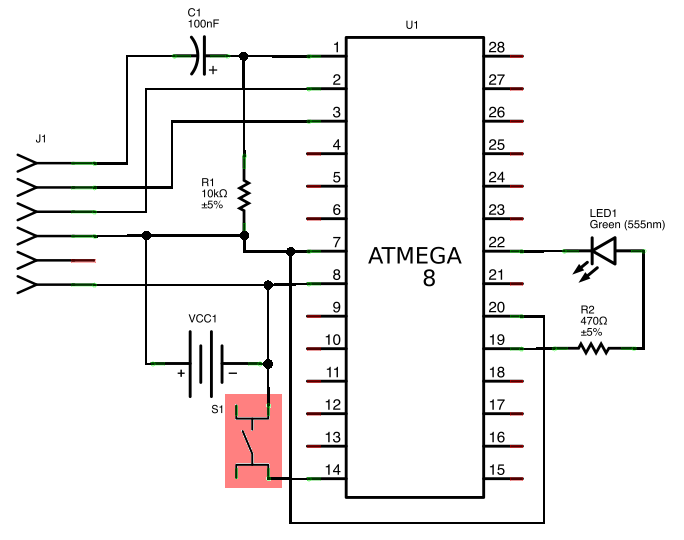
\includegraphics[width=120mm]{LED/S002_get-me-on-get-me-off_Circuit_schema.png}
  \caption{Get me on, get me off - Schema}
  \label{atmega8-get-me-on-get-me-off-schema}
\end{figure}


Second the code


\begin{lstlisting}
; LED/S002_get-me-on-get-me-off.asm

.DEVICE atmega8

.org 0x0000
           rjmp     start

start:
            sbi     DDRB,         5
            cbi     DDRB,         0
            sbi     PORTB,        0

main:
            sbic    PINB,         0
            rjmp    led_on
            cbi     PORTB,        5
            rjmp    led_ok
led_on:
            sbi     PORTB,        5
led_ok:
            rjmp    main
\end{lstlisting}

As you may have guessed, this code represents the 'second form of a standard program'. It does something before the loop - ones - but also does something in the main loop. This program is really busy as we will see in the next program.

The first difference to the former program is, that we use an additional pin/bit. This time for input. To set this pin, bit 0 on port B at pin 14 of the micro controller, to input mode, we send a '0' to its data direction register (DDR). Further we send a '1' to this bit 0 of the port as if we would set the port to output +5V. But this bit is in 'output mode'. In this case, sending '1' to the bit at the port means: 'Switch on the internal pull-up resistor!'

After this, the signal read from this bit is 'ON' or '1'. To interact with the micro controller and change the signal to OFF, we need to pull-down the pin to GND.

If we do so, our program switches the light off as long as we ground bit 0, which does not make real impressive application to boast around with. For us it is great anyway because we understand what happens.

If you follow the programs flow:

\begin{enumerate}
  \item Initialise system and devices
  \item Read bit 0
  \item Set bit 5 accordingly
  \item Start with (2)
\end{enumerate}

You may ask why we permanently output a signal that nearly never changes. Assuming our program reads the input bit one million times per second, a human will not be able to put any business to this program by flipping the switch on and off. If you pick on your signal line as fast as you can then in the eye of your program the signal nearly never changes.

Is there room for optimisation? We believe not.

Are there alternatives? Yes there are!

We could save the output status, compare the status from the input bit with the stored status the light was set to and only change the output signal if the input signal has changed.

This sounds easy, but it is not! It is not only not easy, it is dangerous, costly and complicated. And it is of no use, because you do a lot of commands without any effect.

The concept is dangerous because you may be out of synchronisation with your light. In this case you light may react inverse to your intension or does not react at all.

It is costly not only because the program would be much larger but you need to eat up one CPU register and we only have 32 of them at all.

And it is complicated because you have to synchronise two entities (the light and the status register) to generate one effect. Which is a major risk and drawback.

Because of this, we might be right in our assumption that the developers of our \at micro controller created the chip in such a way that nothing happens if we switch on a bit that is ON already.

Another alternative may be to 'stop' the program as long as it waits for the input signal to change. This may be possible, but it lies far behind our current knowledge.

There is no command that makes the micro controller wait for an input signal. But there are ways to reach a similar effect.

Which means, for now we are out of options and have to stay with the solution as presented in this section. But we will come to status management later.